\section{Introduction}\label{sec:positioningIntroduction}
A autonomous vehicle has as a main function to control all actors on its own.
This means that no human give a sign to the car that now its the time to turn the motor on.
To decide how the single components have to act at which time 
the car need information about its own position which are as good as possible.
This chapter will present some sensors which can be used to get information about the position and rate them in different categories.
Another part of this chapter is to calculate the most possible current position based on the input data of different sensors.


\section{Sensors}
The sensors which were used in a autonoumas vehicle are very important for the final result.
If the sensors are worse the whole vehicle never can bring a good result.
But not only the sensor is important for the behaviour of the car.
Also software which read out the value and filter and correct them is very important.

First the main sensor categories which can be used are listed and then the different rating categories will be explained.
\begin{itemize}
\item absolute sensors
	\subitem lateration
		\subsubitem GPS	
		\subsubitem Mobile telephony
\item environment detection
	\subitem image recognition
	\subitem bumper
	\subitem distance sensor
		\subsubitem ultrasonic
		\subsubitem infrared sensor
\item relative sensors
	\subitem touchless
		\subsubitem gyro sensor
		\subsubitem acceleration
		\subsubitem magnetometer
	\subitem other
		\subsubitem rotary encoder
		\subsubitem mouse sensor
\end{itemize}


\subsection{Output Value Format}
The different types of sensors requires different ways a sensor can return its value.
Mainly the return type can be categorized in analog and digital values.
But this is a very vague grouping because some sensors return values which contain properties of analog and digital values as well.
On the other hand there are sensors which offer their results in two or more interfaces and so they are analog and digital sensors at the same time.


\subsection{Analog}
The most cheap sensors are analog sensors.
This sensors don't need any logic to interpret the result.
The group of analog sensors can be split up in sensors which return a voltage, sensors where the resistor can be measured and sensors which return a current.


\subsection{Analog Current}
Sensors which return a analog current have the problem that they return a very small current.
Examples for analog sensors which return a current are:
\begin{itemize}
\item Photo Diode
\item pH Sensor
\end{itemize}
The photo diode produces a very small amount of energy through the light which get 


\subsection{Analog Voltage}
 


\subsection{Binary}


\subsection{Digital (I2C, UART)}


\subsection{Quadrature Output}


\subsection{Measures Fails, Tolerance, Errors}
\begin{figure}
\makebox[\linewidth]{
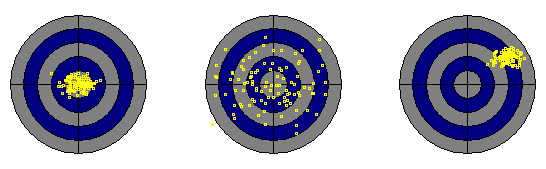
\includegraphics[scale=0.5]{picturesPositioning/precisionDarts.png}
}
\caption{Error Types \cite{img:precisionDarts}}
\label{fig:errorTypes}
\end{figure}
The used sensors have different properties.
One is faster and the another one have a higher precision.
In this section the different types of errors which a sensor can produce are explained.


\subsubsection{Methodical Errors}
Methodical errors are errors which are expectable.
This means the errors have similar properties.
They occurs mainly when devices are badly calibrated.
A example of a methodical error is the right picture of Errors~\ref{fig:errorTypes}.
This example shows that methodical errors are those which are the easiest one to create an algorithm which calculates the real value.
Such a algorithm could be also a simple addition or multiplication.
Also a calibration of the device can help to improve the result.


\subsubsection{Run Away Values}
Run away values are single measure results which doesn't fit in the expected range.
This means that most of the values which are measured are close to the real value except a very small count of values.
A very popular example for a run away value are the red pixels in a photo which was made by a digital camera.
Although the most pixel fit very well there are some pixel which return a value which is to much red.
This effect of digital cameras come through when the image sensor get to hot.
However, this effect that heat increase the error rate is not only by image sensors.
Also other sensors produce much more errors if they become hot.
The type of error which is produced through heat can be very different.
Some sensors lose precision other produce a methodical error.
Often sensors produce combined bugs.


\subsubsection{Brake Down}
A break down is when a sensor lose its full functionally.
The way a brake down can be recogniced could be very different.
The worsest thing which could happen is when device produce a shortbrake because this can also damage the whole car.
This scenario is realy rare.
Most times the device will return a constant value like zero or the digital interface can't be acces any more.
In such a case the software shouldn't hang up.
In a intelligent autonoumas software the car should recognice that the sensor will not react any more and it should stop asking and waiting for the answer.
Instead of the broken sensor the software should chose another sensor which is perhaps not as good as the old one but bether than nothing.


\subsubsection{Bad Precision}
This type of error is that one which is much heavier to handle than other errors.
In case of a bad precission the sensor doesn't return the value as precission as required.
So the returned value can be seen as random number in a defined range of the real value
A possibility to handle this error is to calculate the average value of some meassures.
This method has the disadvantage that short high or low values of the real input dissapears.


\section{Selection of Sensors}



\section{Combine Different Sensors}


\section{Position Specification}
